\FloatBarrier
\section{Methodology}

\begin{figure*}[t]
    \centering
    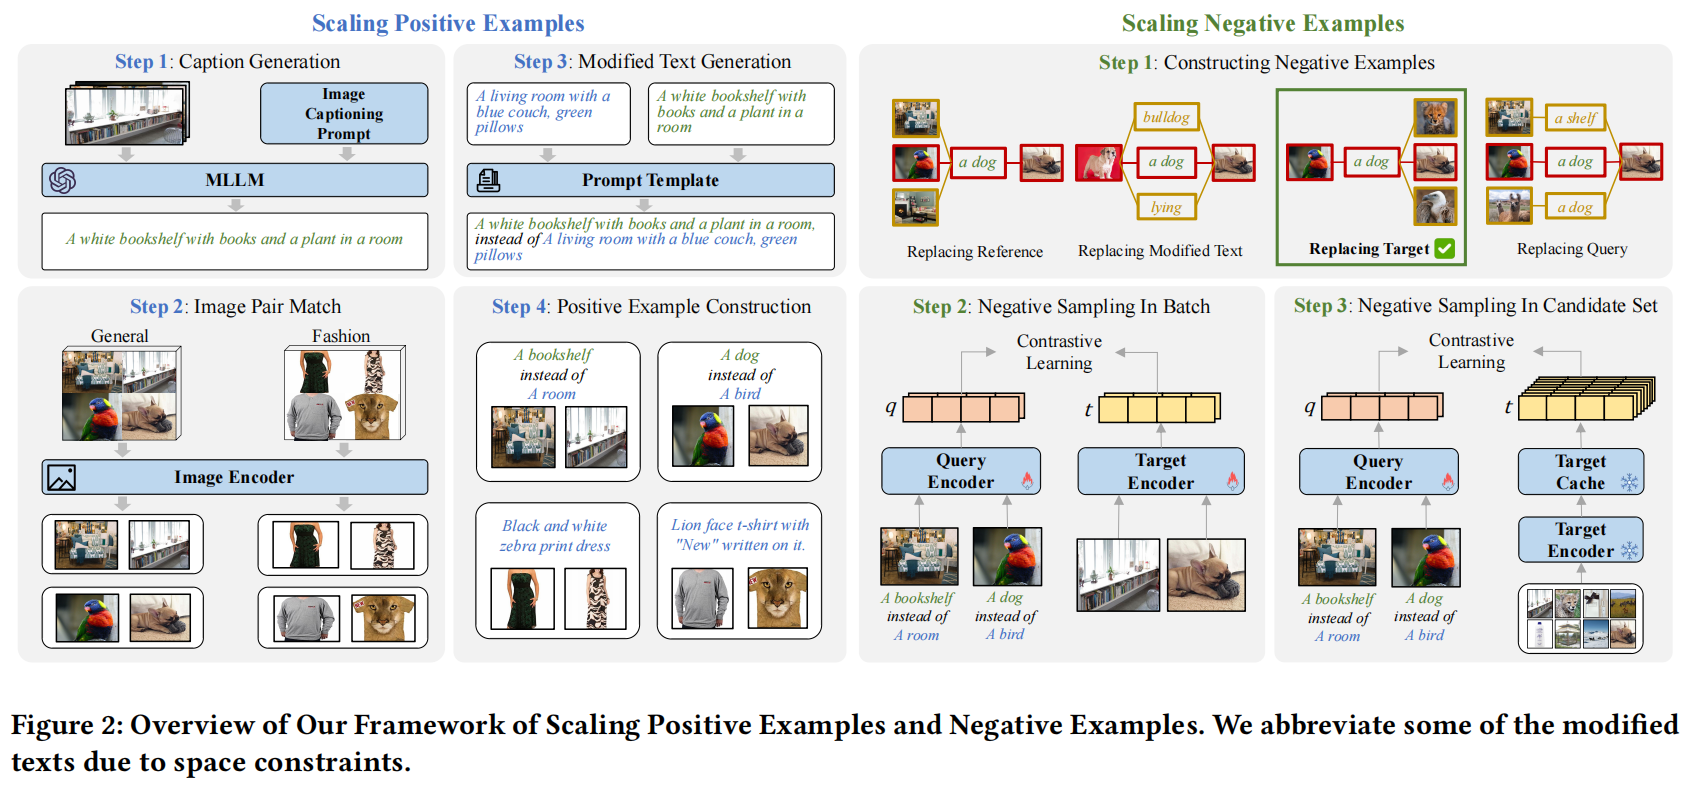
\includegraphics[width=\textwidth]{figures/overview.png}
    \caption{Overview of the methodology.}
    \label{fig:methodology_overview}
\end{figure*}

\subsection{Baselines}

The baselines we used are derived from two key papers. Bai et al., 2023~\cite{bai2023sentencelevelpromptsbenefitcomposed} introduces the initial methodology for composed image retrieval (CIR) using sentence-level prompts. Feng et al., 2024~\cite{feng2024improvingcomposedimageretrieval} presents improvements over the first by leveraging contrastive learning with scaling positives and negatives to enhance CIR performance. Figure~\ref{fig:methodology_overview} provides an overview of the methodology.

\subsubsection{Preliminary}
Suppose a CIR dataset consists of \(N\) annotated triplets consisting of reference images (\(r\)), modified text (\(t\)), and target image (\(t\)). A candidate image set consists of all reference images and target images. The task is to use reference image \(r(i)\) and modified text \(t(i)\) to compose a query \(q(i)\). Then this \(q(i)\) is used to retrieve target images from the candidate set.

\subsubsection{Paradigm of Composed Image Retrieval}
Multiple annotated triplets are combined into a mini-batch, and the reference images and modified texts in the same batch are then encoded using a query encoder to obtain query representations. The target images are encoded using an image encoder to obtain target image representations. The cosine similarity is then adopted to calculate the similarity between the query and target image representations.

\subsubsection{Contrastive Learning}
Treat the annotated examples as positive examples and treat the examples obtained by replacing the target image in the positive examples with another image in the mini-batch as the negatives. This approach pulls the query and target representations in positive examples closer while pushing the query and target representations in negative samples further. This yielded good results; however, the lack of positive examples and negative examples severely limits the full performance of contrastive learning, leading to optimization.

\subsubsection{Scaling Positive Examples}
Using multi-modal Large Language Model (MLLM) to construct the triplets for CIR.

\paragraph{Caption Generation}
Design a prompt template to guide the MLLM to obtain a brief caption for each image under constrained conditions, where \(\text{type}\) and \(k\) are two dataset-specific parameters to simulate the type and length of modified text in the real dataset.

\paragraph{Image Pair Matching}
Match two image-text pairs to generate a quadruplet. Introducing a uni-modal image encoder to get the representation of every image and calculate the pairwise similarity between two different images. Then we can rank the similarities related to the reference image in descending order. Only one image whose similarity rank is between \([c_0, c_1)\) (\(c_0 < c_1\)) will be chosen as the target image, where \(c_0\) and \(c_1\) are two hyperparameters. This forms quadruplets.

\paragraph{Modified Text Generation}
From the quadruplets, design a prompt template that generates modified text by either one of these:
\begin{itemize}
    \item \(P_{\text{temp0}}: \{C_t^i\} \text{ instead of } \{C^i\}\)
    \item \(P_{\text{temp1}}: \text{Unlike } \{C^i\}, \text{I want } \{C_t^i\}\)
    \item \(P_{\text{temp2}}: \{C_t^i\}\)
\end{itemize}

\paragraph{Positive Example Construction}
Combine image pairs from the second step with the modified text obtained in the third step to get new \(M\) triplets.

\subsubsection{Scaling Negative Examples}
Construct negative examples by replacing any element in the triplet. There are four methods to construct negative examples, and the authors examined each method to conclude that replacing the target image will obtain the best negative examples.

\subsubsection{Two-stage Finetuning}
In the first stage, fine-tune both the query encoder and the target encoder with in-batch negative sampling. In the second stage, freeze the target encoder and only fine-tune the query encoder.

\subsection{Potential Approaches}
We aim to improve the baseline model by integrating new techniques and optimizations.

\subsubsection{Image Generation}
One potential approach is to generate images that seamlessly align with the reference image and relative captions. By integrating a new image, we think that the model can incorporate image-side information to improve the performance of the model. We propose to input the reference image and text into the Multi-Instance Generation Controller (MIGC)~\cite{Zhou_2024_CVPR} to generate a new image. This new image can provide useful information that are difficult to express in text at a fine-grained level.

\subsubsection{Two-stage Optimization}
We also propose a two-stage approach to optimize the performance. First, we filter out the candidate images that are not relevant to the reference image and modified text. Then, we use the filtered candidate images to retrieve the target image. This approach can reduce the search space and improve the retrieval performance.
